\section{Use Case Diagram}
\label{sec:UC}

Gli use case dettagliano le interazioni tra attori e sistema a partire dai requisiti funzionali e mantengono riferimenti espliciti agli RF correlati. Ogni use case utilizza un identificatore stabile \texttt{UC-$nn$}, indipendente dagli identificatori \texttt{RF-$nn$}, e indica i requisiti a cui contribuisce. Non esiste una corrispondenza uno-a-uno tra requisiti e use case: uno stesso RF può essere dettagliato da più use case e uno use case può contribuire a più RF.

\subsection*{Attori}
\begin{itemize}[leftmargin=1.4em, itemsep=0.2em]
    \item \textbf{Operatore Tecnico} (attore primario): tecnico del Comune incaricato di consultare il catalogo, costruire gli scenari, eseguire le ottimizzazioni e analizzare risultati e motivazioni.
    \item \textbf{Decisore Comunale} (attore primario): soggetto (amministratore, dirigente o funzionario) che consulta i risultati, le spiegazioni e i confronti a supporto della decisione finale. Nell'attuale prototipo il ruolo coincide con quello dell'Operatore Tecnico, ma i contenuti sono progettati per essere fruiti anche da chi non ha configurato lo scenario.
    \item \textbf{Assistente AI} (attore secondario, opzionale): componente che produce proposte di configurazione a partire da richieste in linguaggio naturale. Non calcola risultati e non applica modifiche.
    \item \textbf{Motore di Ottimizzazione CP-SAT} (attore secondario): sistema che risolve il problema di ottimizzazione combinatoria.
    \item \textbf{Servizio Mappe} (attore secondario): sistema esterno che fornisce le tessere cartografiche utilizzate per la vista geografica degli edifici.
\end{itemize}

\subsection*{Diagrammi}
Le Figure~\ref{fig:uc-dati}, \ref{fig:uc-decisione} e \ref{fig:uc-analisi} riportano i diagrammi dei casi d'uso, raggruppati per area funzionale. I diagrammi sono generati dai sorgenti PlantUML conservati in \texttt{img/src} insieme agli altri asset del documento. Il caso d'uso UC-08 compare in due diagrammi perché è condiviso tra l'area ``scenario e decisione'' e l'area ``analisi e assistenza''.

\begin{figure}[H]
    \centering
    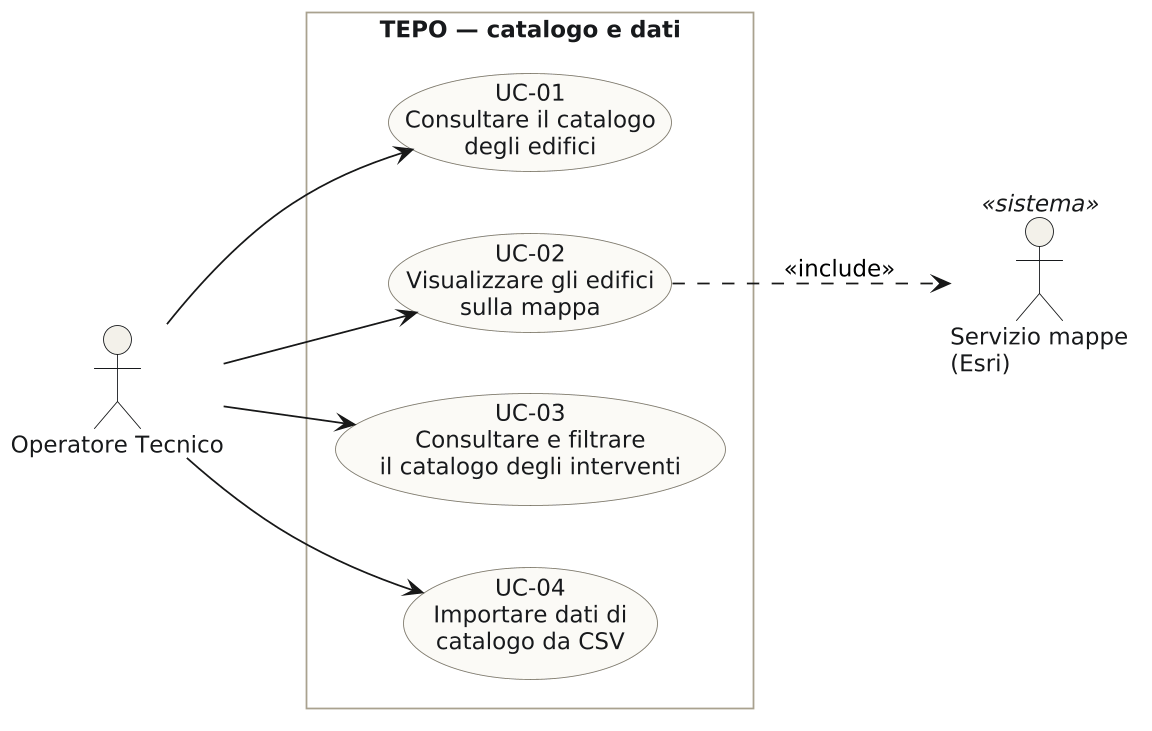
\includegraphics[width=0.92\linewidth]{img/uc-01-dati.png}
    \caption{Casi d'uso dell'area ``catalogo e dati'' (UC-01--UC-04).}
    \label{fig:uc-dati}
\end{figure}

\begin{figure}[H]
    \centering
    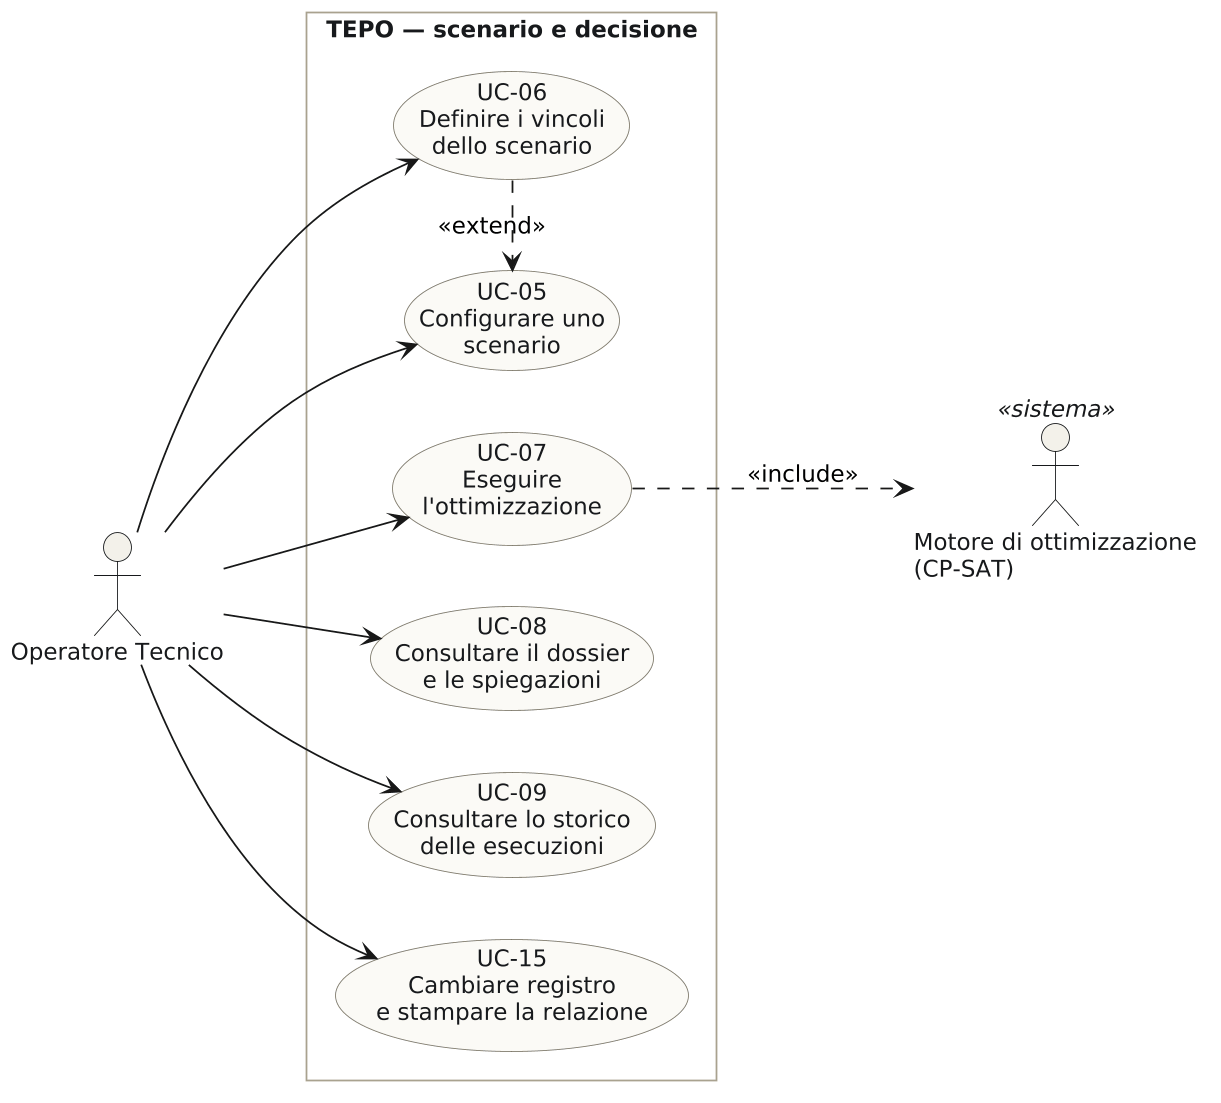
\includegraphics[width=0.92\linewidth]{img/uc-02-decisione.png}
    \caption{Casi d'uso dell'area ``scenario e decisione'' (UC-05--UC-09, UC-15).}
    \label{fig:uc-decisione}
\end{figure}

\begin{figure}[H]
    \centering
    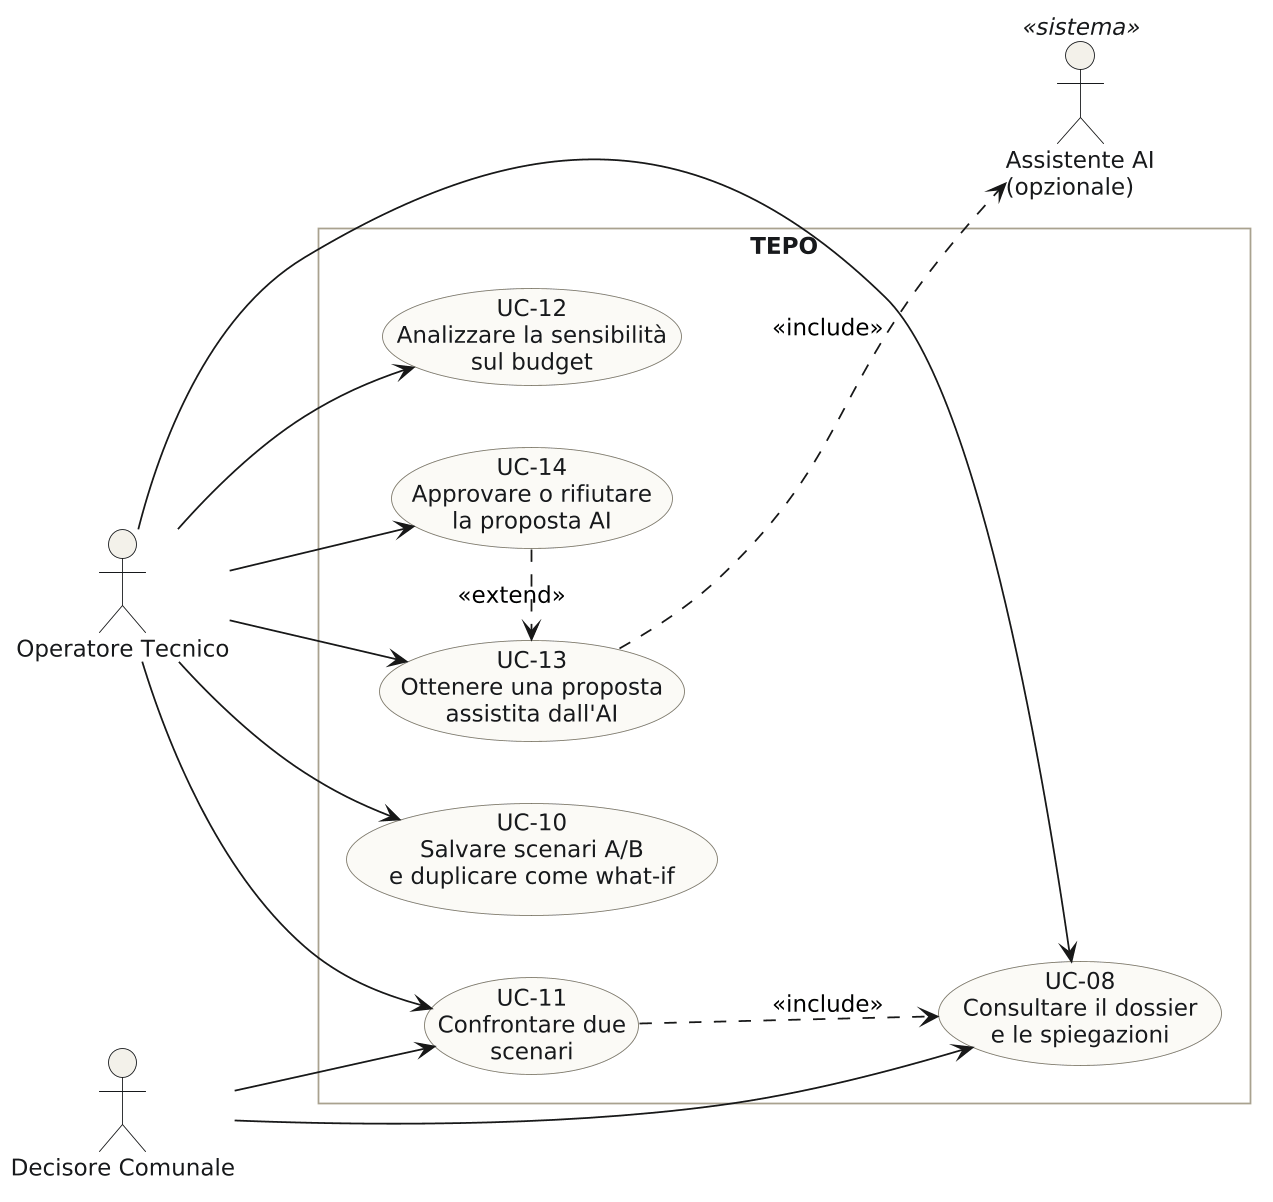
\includegraphics[width=0.92\linewidth]{img/uc-03-analisi.png}
    \caption{Casi d'uso dell'area ``analisi e assistenza'' (UC-08, UC-10--UC-14).}
    \label{fig:uc-analisi}
\end{figure}

\subsection{Descrizione dei casi d'uso}

% ---------------------------------------------------------------- UC-01
\subsection*{Use Case UC-01: Consultare il catalogo degli edifici}
\textbf{Requisiti collegati:} \RFref{rf:catalogo_edifici}, \RFref{rf:provenienza}.\par
\textbf{Attore primario:} Operatore Tecnico.\par
\textbf{Precondizioni:} il catalogo degli edifici è popolato e il servizio dati è raggiungibile.\par
\textbf{Postcondizioni:} l'utente ha consultato l'elenco degli edifici, eventualmente filtrato e ordinato; nessun dato è stato modificato.\par
\textbf{Descrizione:}
\begin{enumerate}[leftmargin=1.6em, itemsep=0.1em]
    \item L'utente apre la pagina ``Edifici''.
    \item Il sistema mostra gli indicatori sintetici del catalogo (edifici, interventi collegati, superficie totale, tipologie rappresentate) e la tabella degli edifici.
    \item L'utente applica uno o più filtri (ricerca testuale, tipologia di edificio) e/o ordina una colonna.
    \item Il sistema aggiorna l'elenco e il contatore ``$N$ di $M$ edifici''.
    \item L'utente consulta, per ciascun edificio, tipologia, superficie, numero di interventi e provenienza del dato.
\end{enumerate}
\textbf{Estensioni:} l'utente può aprire la pagina ``Import'' per importare nuovi edifici (UC-04) oppure la pagina ``Mappa'' per consultare la distribuzione territoriale (UC-02).\par
\textbf{Eccezioni:} se il catalogo è vuoto, il sistema mostra uno stato vuoto con l'azione ``Importa CSV''; se il caricamento fallisce, mostra un messaggio di errore con l'azione ``Riprova''; se i filtri non producono risultati, mostra un messaggio informativo e consente di azzerarli.

% ---------------------------------------------------------------- UC-02
\subsection*{Use Case UC-02: Visualizzare gli edifici sulla mappa}
\textbf{Requisiti collegati:} \RFref{rf:mappa}, \RFref{rf:provenienza}.\par
\textbf{Attori:} Operatore Tecnico (primario); Servizio Mappe (secondario).\par
\textbf{Precondizioni:} il catalogo contiene edifici con coordinate geografiche.\par
\textbf{Postcondizioni:} l'utente ha localizzato gli edifici sul territorio e ne ha eventualmente consultato il dettaglio.\par
\textbf{Descrizione:}
\begin{enumerate}[leftmargin=1.6em, itemsep=0.1em]
    \item L'utente apre la pagina ``Mappa''.
    \item Il sistema mostra la cartografia, i marcatori degli edifici e l'elenco accessibile degli stessi.
    \item Il sistema codifica lo stato di ciascun edificio rispetto all'ultimo risultato tramite colore, contorno e etichetta testuale, e dimensiona il marcatore in base all'investimento.
    \item L'utente cerca un edificio oppure lo seleziona dall'elenco o dalla mappa.
    \item Il sistema mostra il dettaglio dell'edificio: indirizzo, comune, tipologia, superficie, stato e interventi associati.
\end{enumerate}
\textbf{Estensioni:} il cambio di registro (UC-15) aggiorna anche la cartografia di base; l'utente può passare alla pagina ``Interventi'' per filtrare le opzioni dell'edificio selezionato.\par
\textbf{Eccezioni:} se il servizio cartografico non è disponibile, il sistema mantiene utilizzabile l'elenco accessibile degli edifici e segnala il problema; se un edificio non ha coordinate, non compare sulla mappa ma resta nell'elenco.

% ---------------------------------------------------------------- UC-03
\subsection*{Use Case UC-03: Consultare e filtrare il catalogo degli interventi}
\textbf{Requisiti collegati:} \RFref{rf:catalogo_interventi}, \RFref{rf:filtri_interventi}, \RFref{rf:provenienza}.\par
\textbf{Attore primario:} Operatore Tecnico.\par
\textbf{Precondizioni:} il catalogo degli interventi è popolato.\par
\textbf{Postcondizioni:} l'utente ha consultato il sottoinsieme di interventi di interesse; nessun dato è stato modificato.\par
\textbf{Descrizione:}
\begin{enumerate}[leftmargin=1.6em, itemsep=0.1em]
    \item L'utente apre la pagina ``Interventi candidati''.
    \item Il sistema mostra l'elenco completo con edificio, tipologia, costo, risparmi, CO\textsubscript{2}, payback (stima demo), provenienza e stato rispetto all'ultimo risultato.
    \item L'utente combina liberamente i filtri (ricerca testuale, edificio, tipologia, costo minimo e massimo, stato nello scenario).
    \item Il sistema aggiorna elenco, contatori e indicatori del sottoinsieme filtrato; l'utente può ordinare le colonne.
    \item L'utente consulta il dettaglio di un intervento e, se necessario, passa alla configurazione dello scenario.
\end{enumerate}
\textbf{Estensioni:} l'utente può aprire direttamente lo ``Scenario Builder'' (UC-05) per includere gli interventi consultati tra i candidati.\par
\textbf{Eccezioni:} se nessuno scenario è stato eseguito, tutte le opzioni risultano ``Non valutato'' e il sistema lo dichiara; se nessun intervento soddisfa i filtri, mostra un messaggio informativo e consente di azzerarli; se il caricamento fallisce, mostra ``Riprova''.

% ---------------------------------------------------------------- UC-04
\subsection*{Use Case UC-04: Importare dati di catalogo da CSV}
\textbf{Requisiti collegati:} \RFref{rf:import_csv}, \RFref{rf:provenienza}.\par
\textbf{Attore primario:} Operatore Tecnico.\par
\textbf{Precondizioni:} l'utente dispone di un file CSV conforme al formato richiesto.\par
\textbf{Postcondizioni:} le sole righe valide sono state inserite nel catalogo con provenienza sintetica; le righe scartate sono state riportate con la motivazione.\par
\textbf{Descrizione:}
\begin{enumerate}[leftmargin=1.6em, itemsep=0.1em]
    \item L'utente apre la pagina ``Import'' e incolla il contenuto CSV oppure trascina un file.
    \item L'utente avvia la validazione.
    \item Il sistema analizza il contenuto senza scrivere sul database e mostra il riepilogo (righe valide, righe con errori, righe totali) e la tabella degli errori.
    \item L'utente esamina le righe scartate e, se necessario, corregge il CSV e rivalida.
    \item L'utente conferma l'importazione dei soli record validi.
    \item Il sistema inserisce i record, restituisce il numero di record inseriti e scartati, il dettaglio degli scarti e l'eventuale segnalazione di riconciliazione.
\end{enumerate}
\textbf{Estensioni:} l'utente può caricare un contenuto di esempio per verificare il formato; può azzerare il contenuto e ricominciare; al termine può passare alla pagina ``Edifici'' per consultare il catalogo aggiornato.\par
\textbf{Eccezioni:} se l'header è incompleto, il sistema elenca i campi mancanti e non avvia la validazione; se una riga contiene un valore malformato, viene scartata con motivazione esplicita e non convertita in zero; se l'identificativo è duplicato, la riga viene rifiutata; se l'importazione viene richiesta senza una validazione con almeno una riga valida, il sistema la impedisce.

% ---------------------------------------------------------------- UC-05
\subsection*{Use Case UC-05: Configurare uno scenario di ottimizzazione}
\textbf{Requisiti collegati:} \RFref{rf:config_scenario}, \RFref{rf:candidati}, \RFref{rf:scenari_salvati}.\par
\textbf{Attore primario:} Operatore Tecnico.\par
\textbf{Precondizioni:} il catalogo degli edifici e degli interventi è popolato; l'utente ha accesso allo Scenario Builder.\par
\textbf{Postcondizioni:} lo scenario corrente contiene un budget valido, un obiettivo selezionato, un insieme non vuoto di candidati e un insieme di vincoli ben formati; lo scenario è pronto per l'ottimizzazione.\par
\textbf{Descrizione:}
\begin{enumerate}[leftmargin=1.6em, itemsep=0.1em]
    \item L'utente apre la pagina ``Scenario''.
    \item Il sistema mostra i parametri correnti e il riepilogo dello scenario.
    \item L'utente sceglie se e in quale slot (A o B) salvare il risultato.
    \item L'utente inserisce il budget complessivo e seleziona l'obiettivo tra risparmio energetico, risparmio economico e riduzione di CO\textsubscript{2}.
    \item L'utente seleziona gli interventi candidati tramite ricerca, selezione puntuale, ``Seleziona tutti''/``Deseleziona tutti'' o ``Carica set demo''.
    \item L'utente consulta e, se previsto, definisce i vincoli dello scenario (UC-06).
    \item Il sistema aggiorna il riepilogo con costo selezionato, budget e residuo e segnala l'eventuale superamento del budget.
    \item L'utente conferma con ``Ottimizza portafoglio'' oppure torna alla dashboard senza salvare.
\end{enumerate}
\textbf{Estensioni:}
\begin{enumerate}[leftmargin=1.6em, itemsep=0.1em]
    \item L'utente può richiedere una proposta all'assistente AI (UC-13) e applicarla solo dopo approvazione esplicita (UC-14).
    \item L'utente può partire da uno scenario salvato e duplicarlo come what-if (UC-10).
    \item L'utente può caricare il set dimostrativo di nove candidati con budget e obiettivo predefiniti per la demo.
\end{enumerate}
\textbf{Eccezioni:} se il budget non è valido o non è stato selezionato alcun obiettivo o candidato, il sistema impedisce l'ottimizzazione e indica il campo da correggere; se il costo selezionato supera il budget, il sistema avvisa che il portafoglio potrebbe risultare inammissibile senza bloccare la configurazione; se il catalogo non è disponibile, mostra un errore con ``Riprova''.

% ---------------------------------------------------------------- UC-06
\subsection*{Use Case UC-06: Definire i vincoli dello scenario}
\textbf{Requisiti collegati:} \RFref{rf:vincoli_scenario}.\par
\textbf{Attore primario:} Operatore Tecnico.\par
\textbf{Precondizioni:} lo scenario corrente contiene almeno due candidati; l'utente si trova nello Scenario Builder.\par
\textbf{Postcondizioni:} i vincoli applicati sono visibili e coerenti; lo scenario può essere ottimizzato nel rispetto dei vincoli.\par
\textbf{Descrizione:}
\begin{enumerate}[leftmargin=1.6em, itemsep=0.1em]
    \item L'utente apre la sezione ``Vincoli applicati''.
    \item Il sistema mostra i vincoli correnti raggruppati per tipo (incompatibilità, prerequisiti, numero massimo, inclusioni ed esclusioni).
    \item L'utente aggiunge una coppia di opzioni incompatibili, una relazione di prerequisito, un limite numerico su un sottoinsieme oppure un'inclusione o esclusione obbligatoria.
    \item Il sistema valida il vincolo rispetto al catalogo e allo scenario e lo mostra nella lista.
    \item L'utente può rimuovere un vincolo precedentemente aggiunto.
\end{enumerate}
\textbf{Estensioni:} se un vincolo rende il problema inammissibile, il sistema lo segnala e propone la diagnostica; l'utente può rimuoverlo e rieseguire l'ottimizzazione.\par
\textbf{Nota di realizzazione:} nel prototipo demo i vincoli sono precaricati e mostrati in sola lettura; le interazioni descritte rappresentano il comportamento previsto dalla baseline e saranno allineate nel D2.
\textbf{Eccezioni:} se la stessa opzione risulta contemporaneamente inclusa ed esclusa, il sistema rifiuta il salvataggio con un messaggio specifico; se viene introdotto un ciclo di prerequisiti, il sistema lo segnala; se il numero massimo non è positivo o fa riferimento a opzioni inesistenti, il vincolo viene rifiutato; se i vincoli vengono modificati dopo un'ottimizzazione, il risultato precedente non è più valido per lo scenario corrente e il sistema lo rende evidente.

% ---------------------------------------------------------------- UC-07
\subsection*{Use Case UC-07: Eseguire l'ottimizzazione}
\textbf{Requisiti collegati:} \RFref{rf:ottimizzazione}, \RFref{rf:storico}.\par
\textbf{Attori:} Operatore Tecnico (primario); Motore di Ottimizzazione CP-SAT (secondario).\par
\textbf{Precondizioni:} lo scenario corrente è completo e coerente (UC-05 concluso con successo).\par
\textbf{Postcondizioni:} il sistema ha prodotto un risultato con stato esplicito, lo ha registrato nello storico e lo ha reso disponibile nel dossier; in caso di stato non risolutivo, ha comunicato la diagnostica.\par
\textbf{Descrizione:}
\begin{enumerate}[leftmargin=1.6em, itemsep=0.1em]
    \item L'utente richiede l'esecuzione dell'ottimizzazione.
    \item Il sistema valida nuovamente lo scenario e costruisce il payload del problema.
    \item Il sistema invoca il motore di ottimizzazione e mostra lo stato di avanzamento senza bloccare l'interfaccia.
    \item Il motore restituisce una soluzione con lo stato del calcolo, l'eventuale prova di ottimalità e l'esito del tie-break.
    \item Il sistema calcola le spiegazioni deterministiche per ciascuna opzione candidata.
    \item Il sistema calcola l'hash canonico, registra l'esecuzione nello storico ai fini di audit e applica il salvataggio opzionale in A o B.
    \item Il sistema apre il dossier del risultato (UC-08).
\end{enumerate}
\textbf{Estensioni:} in caso di più soluzioni ottime equivalenti, il sistema applica i criteri di spareggio deterministici (minimizzazione del costo, minimizzazione del numero di interventi, preferenza per identificativi crescenti) e ne dà evidenza nel dossier; se l'utente ha scelto uno slot, il risultato viene salvato prima della navigazione.\par
\textbf{Eccezioni:} se il problema è inammissibile, il sistema mostra lo stato ``Nessuna soluzione ammissibile'' con la diagnostica sulle possibili cause; se il calcolo supera il tempo massimo, mostra ``Indeterminato per timeout'' e non presenta alcun portafoglio come definitivo; se l'input non è conforme, mostra ``Modello non valido''; se la chiamata di rete fallisce, mostra un errore con la possibilità di riprovare senza duplicare il risultato.

% ---------------------------------------------------------------- UC-08
\subsection*{Use Case UC-08: Consultare il dossier di risultato e le spiegazioni}
\textbf{Requisiti collegati:} \RFref{rf:risultati}, \RFref{rf:spiegazioni}, \RFref{rf:provenienza}.\par
\textbf{Attori:} Operatore Tecnico (primario); Decisore Comunale (primario, fruitore dei contenuti).\par
\textbf{Precondizioni:} esiste un ultimo risultato disponibile nella sessione.\par
\textbf{Postcondizioni:} l'utente ha letto il portafoglio proposto, gli indicatori, le motivazioni e l'audit del calcolo; il risultato non è stato modificato.\par
\textbf{Descrizione:}
\begin{enumerate}[leftmargin=1.6em, itemsep=0.1em]
    \item L'utente apre la pagina ``Risultato''.
    \item Il sistema mostra l'audit strip (esecuzione, hash del problema, istante, stato del solver, ottimalità, tie-break).
    \item Il sistema mostra gli indicatori aggregati, l'impiego del budget e l'allocazione dell'investimento per edificio.
    \item Il sistema mostra la tabella degli interventi selezionati con la motivazione di ciascuno.
    \item L'utente apre la sezione ``Perché questa soluzione?'', consulta il riepilogo per famiglia di causa ed esplora le motivazioni delle opzioni escluse con filtri e ricerca.
    \item L'utente può salvare il risultato in A o B (UC-10), aprire il confronto (UC-11) o stampare la relazione (UC-15).
\end{enumerate}
\textbf{Estensioni:} l'utente può duplicare uno scenario A o B come what-if e tornare allo Scenario Builder per una nuova configurazione; può filtrare le motivazioni per ``Barriere locali'', ``Causa non determinata'' e ``Selezionati''; può esportare la relazione tramite la stampa del browser.\par
\textbf{Eccezioni:} se non esiste alcun risultato, il sistema mostra uno stato vuoto con l'azione ``Configura uno scenario''; se il risultato è stato prodotto con uno stato non ottimo, il dossier lo evidenzia e invita a leggerne la diagnostica; se i dati di audit non sono disponibili, il sistema mostra i campi mancanti senza inventarli.

% ---------------------------------------------------------------- UC-09
\subsection*{Use Case UC-09: Consultare lo storico delle esecuzioni}
\textbf{Requisiti collegati:} \RFref{rf:storico}, \RNFref{rnf:tracciabilita}.\par
\textbf{Attore primario:} Operatore Tecnico.\par
\textbf{Precondizioni:} è stata eseguita almeno un'ottimizzazione.\par
\textbf{Postcondizioni:} l'utente ha consultato le esecuzioni registrate; nessuna esecuzione è stata modificata.\par
\textbf{Descrizione:}
\begin{enumerate}[leftmargin=1.6em, itemsep=0.1em]
    \item L'utente apre la ``Dashboard''.
    \item Il sistema mostra il registro delle esecuzioni dello scenario con istante, esito, obiettivo, identificativo e investimento.
    \item L'utente consulta l'esecuzione registrata; il dettaglio completo del risultato è disponibile nel dossier dell'ultimo risultato e, per tutte le esecuzioni, tramite le API.
    \item Il sistema espone i dati di audit in sola lettura e non consente di modificare o cancellare le esecuzioni dall'interfaccia.
\end{enumerate}
\textbf{Estensioni:} l'utente può usare il registro per riconoscere un'esecuzione precedente e ricostruirne il contesto prima di un nuovo calcolo; le analisi di sensibilità non compaiono nel registro.\par
\textbf{Eccezioni:} se non esistono esecuzioni, il sistema mostra ``Nessuna esecuzione registrata''; se il registro non è raggiungibile, mostra un errore con ``Riprova'' senza compromettere l'ultimo risultato disponibile.

% ---------------------------------------------------------------- UC-10
\subsection*{Use Case UC-10: Salvare scenari A/B e duplicare come what-if}
\textbf{Requisiti collegati:} \RFref{rf:scenari_salvati}.\par
\textbf{Attore primario:} Operatore Tecnico.\par
\textbf{Precondizioni:} esiste un risultato da salvare oppure uno scenario configurato con uno slot selezionato.\par
\textbf{Postcondizioni:} uno o entrambi gli slot contengono un risultato; gli slot sono visibili nella sessione e richiamabili come what-if.\par
\textbf{Descrizione:}
\begin{enumerate}[leftmargin=1.6em, itemsep=0.1em]
    \item L'utente sceglie lo slot (A o B) dal selettore ``Salva come'' nello Scenario Builder oppure dai comandi del dossier.
    \item Il sistema salva il risultato nello slot scelto e ne aggiorna la rappresentazione nella sessione.
    \item L'utente consulta l'occupazione degli slot e l'importo salvato nel pannello ``Sessione A/B''.
    \item L'utente richiede di duplicare uno slot come what-if.
    \item Il sistema apre lo Scenario Builder con i parametri del risultato salvato, senza modificare l'originale.
\end{enumerate}
\textbf{Estensioni:} l'utente può sovrascrivere uno slot occupato; il sistema salva il nuovo risultato e mostra una conferma non bloccante. L'utente può azzerare l'intera sessione (slot e ultimo risultato) previa conferma.\par
\textbf{Eccezioni:} se l'archiviazione della sessione non è disponibile, il sistema segnala che il salvataggio non è possibile e mantiene i dati correnti; se l'utente annulla la conferma di sovrascrittura, lo slot resta invariato.

% ---------------------------------------------------------------- UC-11
\subsection*{Use Case UC-11: Confrontare due scenari}
\textbf{Requisiti collegati:} \RFref{rf:confronto}.\par
\textbf{Attori:} Operatore Tecnico (primario); Decisore Comunale (primario).\par
\textbf{Precondizioni:} entrambi gli slot A e B sono popolati.\par
\textbf{Postcondizioni:} l'utente ha letto i parametri, gli indicatori e gli scostamenti tra i due scenari.\par
\textbf{Descrizione:}
\begin{enumerate}[leftmargin=1.6em, itemsep=0.1em]
    \item L'utente apre la pagina ``Confronto''.
    \item Il sistema mostra i due scenari affiancati con i parametri e gli indicatori.
    \item Il sistema mostra gli scostamenti calcolati come $B - A$ per investimento, risparmio energetico, risparmio economico, CO\textsubscript{2} e numero di interventi.
    \item Il sistema mostra la tabella delle metriche e gli elenchi degli interventi aggiunti in B e rimossi rispetto ad A.
    \item Se gli obiettivi sono diversi, il sistema mostra l'avviso di non omogeneità.
    \item L'utente può tornare al dossier dell'ultimo risultato o stampare il confronto.
\end{enumerate}
\textbf{Estensioni:} l'utente può duplicare lo scenario A o B come what-if per costruire una terza alternativa.\par
\textbf{Eccezioni:} se uno o entrambi gli slot sono vuoti, il sistema mostra ``Servono due scenari salvati'' e le azioni per completarli; se i dati di uno scenario non sono disponibili, il sistema mostra i valori mancanti senza inventarli.

% ---------------------------------------------------------------- UC-12
\subsection*{Use Case UC-12: Analizzare la sensibilità sul budget}
\textbf{Requisiti collegati:} \RFref{rf:sensibilita}.\par
\textbf{Attore primario:} Operatore Tecnico.\par
\textbf{Precondizioni:} il catalogo è disponibile; l'utente ha accesso alla pagina ``Sensibilità''.\par
\textbf{Postcondizioni:} l'utente ha eseguito lo sweep e ha letto la sintesi, l'andamento dell'obiettivo e la stabilità delle selezioni.\par
\textbf{Descrizione:}
\begin{enumerate}[leftmargin=1.6em, itemsep=0.1em]
    \item L'utente apre la pagina ``Sensibilità''.
    \item Il sistema mostra la nota metodologica e il form con budget base, obiettivo, numero di punti e fattori minimo e massimo.
    \item L'utente seleziona i candidati dello sweep.
    \item L'utente avvia l'analisi.
    \item Il sistema esegue una sequenza deterministica di ottimizzazioni, una per ciascun punto, e mostra la sintesi (punti analizzati, sempre selezionati, oscillanti, mai selezionati).
    \item L'utente consulta l'andamento dell'obiettivo, la mappa di selezione per budget, i risultati per punto e la sezione ``Stabilità delle selezioni''.
\end{enumerate}
\textbf{Estensioni:} l'utente può selezionare o deselezionare tutti i candidati e modificare ampiezza e densità della griglia entro i limiti previsti; la nota metodologica chiarisce che l'analisi non è una simulazione Monte Carlo.\par
\textbf{Eccezioni:} se il numero di punti non è compreso tra 3 e 51 o i fattori non sono validi, il sistema impedisce l'avvio e indica il vincolo; se un punto non conclude, il sistema ne mostra lo stato senza interrompere l'analisi; se la rete fallisce, mostra un errore con la possibilità di riprovare.

% ---------------------------------------------------------------- UC-13
\subsection*{Use Case UC-13: Ottenere una proposta assistita dall'AI}
\textbf{Requisiti collegati:} \RFref{rf:ai_proposta}.\par
\textbf{Attori:} Operatore Tecnico (primario); Assistente AI (secondario, opzionale).\par
\textbf{Precondizioni:} l'utente si trova nello Scenario Builder.\par
\textbf{Postcondizioni:} il sistema ha mostrato una proposta di configurazione non applicata, corredata di origine, motivazione, eventuali informazioni mancanti e avvertenze.\par
\textbf{Descrizione:}
\begin{enumerate}[leftmargin=1.6em, itemsep=0.1em]
    \item L'utente apre il pannello ``Assistente AI''.
    \item Il sistema mostra lo stato dell'integrazione (``LLM attivo'', ``Modalità locale'' oppure ``Stato AI non disponibile'') e le note del provider.
    \item L'utente descrive lo scenario desiderato in linguaggio naturale e invia la richiesta.
    \item Il sistema inoltra la richiesta al motore a regole oppure, se configurato, al modello linguistico esterno.
    \item Il sistema mostra la proposta con budget, obiettivo, candidati proposti, motivazione, origine e segnalazioni.
\end{enumerate}
\textbf{Estensioni:} se il modello esterno non è raggiungibile o restituisce una risposta non conforme, il sistema ricade sul motore a regole e lo segnala con l'indicazione ``LLM (fallback locale)''; l'utente può consultare le note del provider per capire perché l'LLM non è attivo.\par
\textbf{Eccezioni:} se la richiesta è vuota, il sistema non la invia; se il provider non è configurato, la proposta viene comunque prodotta localmente; se la proposta contiene identificativi sconosciuti, il sistema li filtra e avverte l'utente; se la chiamata fallisce, il sistema mostra un errore e non modifica lo scenario.

% ---------------------------------------------------------------- UC-14
\subsection*{Use Case UC-14: Approvare o rifiutare la proposta AI}
\textbf{Requisiti collegati:} \RFref{rf:ai_approvazione}.\par
\textbf{Attore primario:} Operatore Tecnico.\par
\textbf{Precondizioni:} il sistema ha prodotto una proposta AI visibile nel pannello.\par
\textbf{Postcondizioni:} la proposta è stata applicata con un atto esplicito oppure rifiutata; in caso di rifiuto lo scenario è invariato.\par
\textbf{Descrizione:}
\begin{enumerate}[leftmargin=1.6em, itemsep=0.1em]
    \item L'utente esamina la proposta e le sue segnalazioni.
    \item Il sistema ricorda che la proposta non è stata applicata e che richiede revisione umana.
    \item L'utente sceglie ``Applica allo scenario'' oppure ``Rifiuta''.
    \item In caso di applicazione, il sistema aggiorna budget, obiettivo e selezione dei candidati, mostra l'avviso di verifica e lascia all'utente il comando ``Ottimizza portafoglio''.
    \item In caso di rifiuto, il sistema elimina la proposta e lascia invariato lo scenario.
\end{enumerate}
\textbf{Estensioni:} dopo l'applicazione l'utente può correggere manualmente i parametri proposti prima di ottimizzare; le opzioni che la proposta suggerisce di escludere restano selezionate ma vengono evidenziate.\par
\textbf{Eccezioni:} se la proposta contiene un budget non valido, il sistema non la applica e mostra l'errore; se l'utente chiude il pannello senza scegliere, la proposta non viene applicata.

% ---------------------------------------------------------------- UC-15
\subsection*{Use Case UC-15: Cambiare registro e stampare la relazione}
\textbf{Requisiti collegati:} \RFref{rf:tema}, \RFref{rf:risultati}.\par
\textbf{Attore primario:} Operatore Tecnico.\par
\textbf{Precondizioni:} l'utente si trova in una pagina dell'applicazione.\par
\textbf{Postcondizioni:} il registro visivo è stato cambiato e conservato, oppure la relazione è stata inviata alla stampa con fondo chiaro e inchiostro scuro.\par
\textbf{Descrizione:}
\begin{enumerate}[leftmargin=1.6em, itemsep=0.1em]
    \item L'utente attiva il comando di cambio registro nella fascia di stato oppure dalla palette dei comandi rapidi.
    \item Il sistema applica il registro scelto (``Relazione'' o ``Sala operativa'') mantenendo invariato il layout e l'informazione.
    \item Il sistema conserva la scelta per le sessioni successive e usa la preferenza del sistema operativo alla prima apertura.
    \item L'utente richiede la stampa della relazione dal dossier del risultato o dal confronto.
    \item Il sistema prepara la stampa con fondo chiaro e inchiostro scuro, nascondendo navigazione e controlli e mantenendo leggibili tabelle e pannelli.
\end{enumerate}
\textbf{Estensioni:} il registro può essere cambiato anche dalla palette dei comandi rapidi; la stampa può essere annullata dall'utente nel dialogo del browser.\par
\textbf{Eccezioni:} se l'archiviazione locale non è disponibile, il sistema usa la preferenza del sistema operativo per la sessione corrente; se non è disponibile un risultato o un confronto, il comando di stampa del dossier non è mostrato, mentre il comando rapido di stampa resta disponibile e stampa la pagina corrente.
